\newpage

\changeindent{0cm}
\section{実験}
\changeindent{2cm}

%%%%%%%%%%%%%%%%%%%%%%%%%%%%%%
% 4.1 実験 1 
% 4.2 実験 2
%%%%%%%%%%%%%%%%%%%%%%%%%%%%%%

本章では,本研究で取り組んだ実験について記述する.

\subsection{実験 1}

最初に,文章の話題ごとに皮肉か非皮肉かを推定する実験に取り組んだ.
モデルには BERT を使用し,データセットには SARC 2.0 main balanced データセットを使用した.
\par
まず subreddit ごとにデータを抽出し,新たに実験用データセットを構築した.
その際にテストデータが 1,500 件以上取得できたものを選択し,politics \footnote{\url{https://www.reddit.com/r/politics/}},AskReddit \footnote{\url{https://www.reddit.com/r/AskReddit/}},worldnews \footnote{\url{https://www.reddit.com/r/worldnews/}},pcmasterrace \footnote{\url{https://www.reddit.com/r/pcmasterrace/}} の 4 つの subreddit のデータセットを実験に使用した.
各 subreddit はそれぞれ,politics は米国の時事ニュースや政治的なニュースを,AskReddit はユーザ同士の質問や回答のやりとりを,worldnews は米国以外の時事ニュースや政治的なニュースを,pcmasterrace はコンピュータやゲームに関する話題を扱っている.
比較のため,全ての subreddit からランダムにデータをサンプリングした random データセットを構築し,こちらも実験に使用した.
このとき同じ親投稿を持つ皮肉データと非皮肉データのペアは崩さないように抽出した.
random データセットに含まれる subreddit を確認したところ,訓練データは 1,257 種類,テストデータは 569 種類の subreddit から構成されていた.
表 \ref{tb:4_subreddit_data} に各データセットのデータ数を示す.
なお各データセットには皮肉データと非皮肉データは同数含まれている.

%%% table
\begin{table}[b]
  \caption{各データセットのデータ数}
  \label{tb:4_subreddit_data}
  \centering
  \begin{tabular}{c c c} \hline

データセット & 訓練 (件) & テスト (件) \\ \hline
politics & 13,668 & 3,406 \\
AskReddit & 11,660 & 3,006 \\
worldnews & 9,444 & 2,246 \\
pcmasterrace & 7,400 & 1,772 \\
random & 14,000 & 3,500 \\ \hline

  \end{tabular}
\end{table}
% end

\par
図 \ref{fig:40_model} にモデルの概要を示す.
まず入力の先頭に [CLS] トークンを,各コメントの末尾に [SEP] トークンを付けて BERT に入力し,分散表現を取得した.
分散表現のうち,文頭の [CLS] トークンに該当する分散表現を線形層に入力して,皮肉か非皮肉かで二値分類した.
訓練データでモデルを学習し,テストデータでその性能を評価した.
評価指標には Accuracy(正解率),Precision(適合率),Recall(再現率),F1 値を使用した.

% figure model
 \begin{figure}[tb]
 	\begin{center}
	 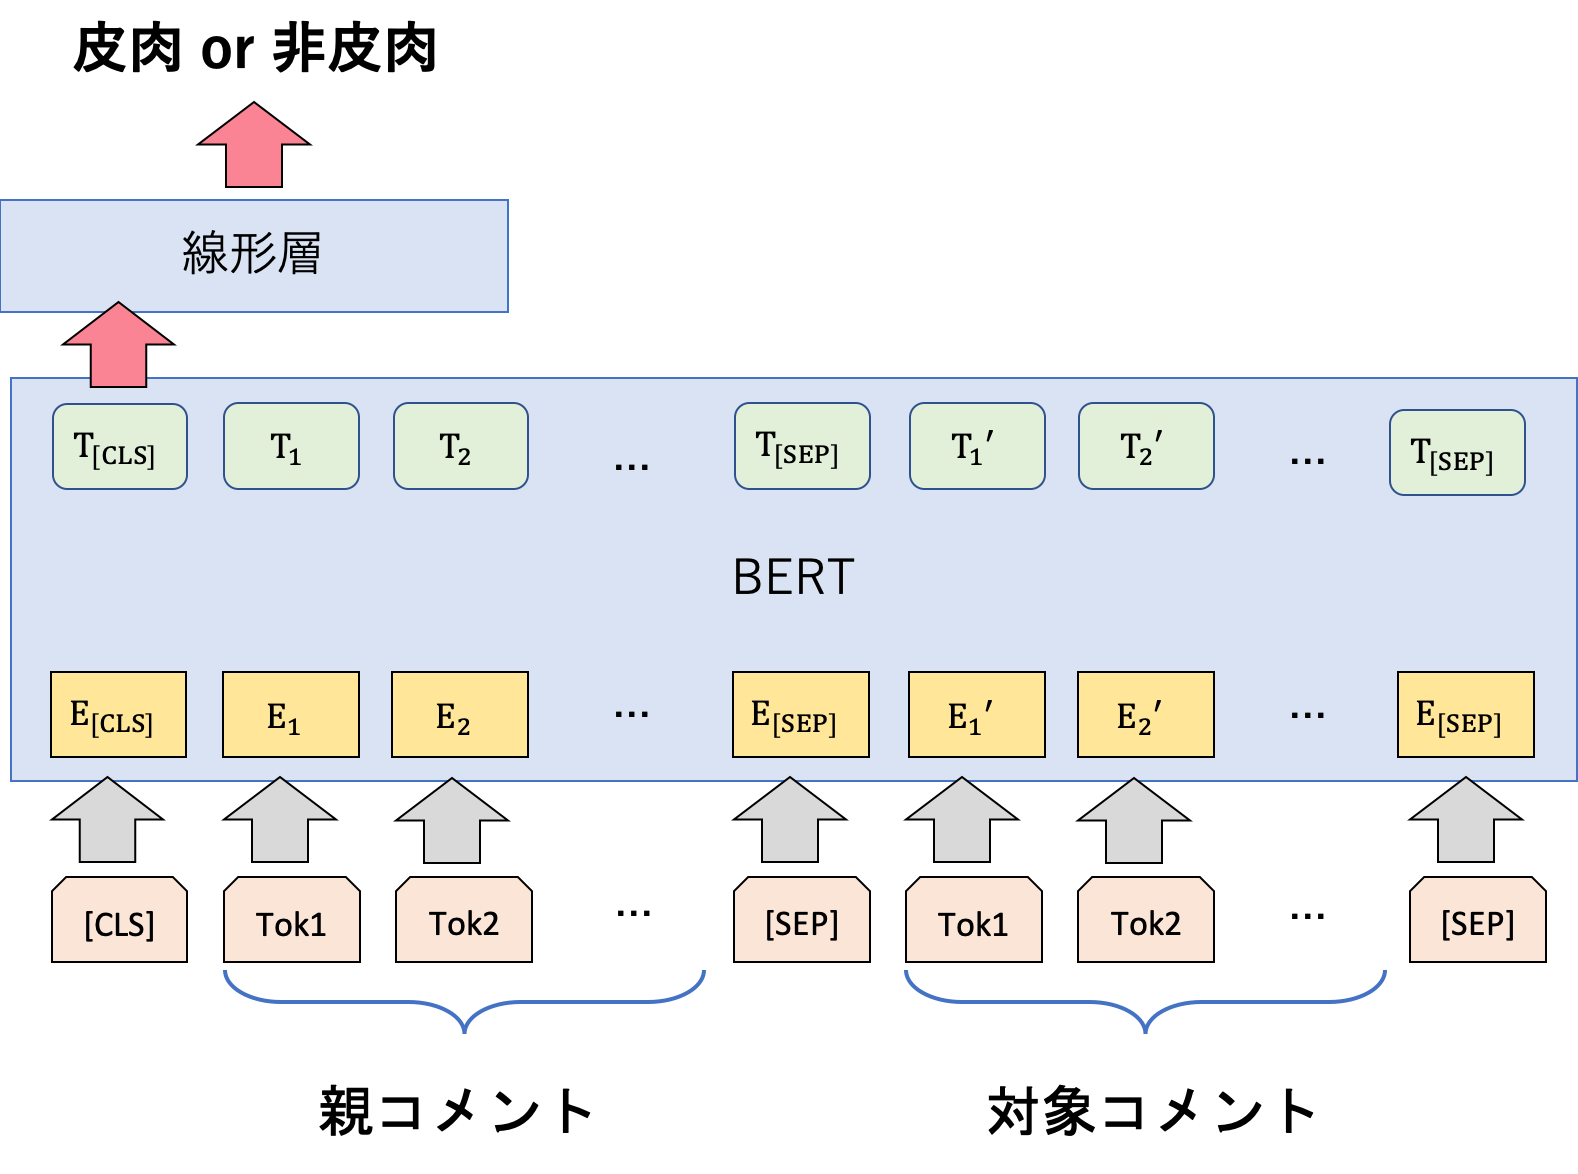
\includegraphics[width=0.8\linewidth]{./figure/40_model.png}
	 \end{center}
 \caption{実験モデルの概要}
 \label{fig:40_model}
 \end{figure}
% end figure


表 \ref{tb:4_bert_param} に実験のパラメータを示す.
BERT と線形層の学習率は予備実験によって値の範囲を定め,Optuna によって探索した.
目的関数にはテスト時の Accuracy を設定し,この値を最大化するように探索した.
学習時は BERT の全層をファインチューニングし,線形層も重みを更新した.
\par

%%% table
\begin{table}[tb]
  \caption{実験パラメータ}
  \label{tb:4_bert_param}
  \centering
  \begin{tabular}{c c} \hline

\multicolumn{2}{c}{BERT} \\ \hline
モデル & bert-base-uncased \\ 
入力層次元数 & 512 \\
出力層次元数 & 768 \\
学習率(探索範囲) & $1 \times 10^{-6}$ 〜 $1 \times 10^{-4}$ \\ \hline
\multicolumn{2}{c}{線形層} \\ \hline
入力層次元数 & 768 \\
出力層次元数 & 2 \\
学習率(探索範囲) & $1 \times 10^{-6}$ 〜 $1 \times 10^{-4}$ \\ \hline
\multicolumn{2}{c}{学習} \\ \hline
エポック数 & 20 \\
バッチサイズ & 16 \\
損失関数 & Cross Entropy Loss \\
最適化関数 & Adam \\
 & $\left( 
 \begin{tabular}{c}
 \footnotesize{learning rate = 0.001} \\ \footnotesize{$\beta_1 = 0.9$, $\beta_2 = 0.999$}
 \end{tabular}
  \right)$ 
%最適化関数 & 
%	\begin{tabular}{c}
%	Adam \\ learning rate $= 0.001$ \\ $\beta_1 = 0.9$, $\beta_2 = 0.999$
%	\end{tabular}

\\ \hline
  \end{tabular}
\end{table}
% end



%%%%%%%%%%%%%%%%%%%%%%%%%%%%%%
%\afterpage{\clearpage}
\subsection{結果と考察}
表 \ref{tb:4_bert_result} に実験結果を示す.
太字の項目はベースラインである random データセットでの評価値を上回ったことを表している.
表より random データセットでの評価値を上回った項目が多いことが分かる.
このことは,subreddit ごとに皮肉推定をすることが,推定精度向上に有効に働いていると考えられる.
また politics データセットでは全ての評価指標で random データセットでの皮肉推定精度を上回った.
一方で AskReddit データセットでは全ての評価指標で random データセットでの皮肉推定精度を下回った.
このことから,politics データセットの皮肉表現の特徴を上手く捉えることができ,正しく推定できていると考えられる.
反対に,AskReddit データセットは何らかの理由で皮肉推定が困難であったと考えられる.
その理由としては以下のことが考えられる.
\begin{itemize}
	\setlength{\itemsep}{-1mm}
\item 皮肉文章と非皮肉文章が類似している
\item 含まれる話題が多く,学習によって捉えきれない
\item 皮肉・非皮肉ラベル付けが適切でない
\item 訓練データとテストデータの違いが大きい
\end{itemize}


%%% table
\begin{table}[tb]
  \caption{実験結果(実験 1) }
  \label{tb:4_bert_result}
  \centering
  \begin{tabular}{c c c c c} \hline

dataset & Accuracy & Precision & Recall & F1 score  \\ \hline
politics & \textbf{0.730} & \textbf{0.722} & \textbf{0.748} & \textbf{0.735} \\
AskReddit & 0.619 & 0.630 & 0.580 & 0.604 \\
worldnews & \textbf{0.690} & 0.655 & \textbf{0.803} & \textbf{0.721} \\
pcmasterrace & 0.648 & 0.635 & \textbf{0.698}  & \textbf{0.665} \\ \hline
random & 0.653 & 0.664 & 0.618 & 0.640 \\ \hline

  \end{tabular}
\end{table}
% end


また worldnews データセットでは Recall の値が高くなった.
このことは,データセットに含まれる皮肉データに対して皮肉であると正しく予測したものが多いことを表している.
反対に,Precision の値は random データセットでの評価値を下回り,このことは,皮肉であると予測したデータのうち真のラベルが皮肉であったものが少なかったことを表している.
すなわち,真のラベルが非皮肉であるものに対して皮肉であると予測したものが多いことを意味している.




